%\documentclass[12pt]{article}
%\usepackage[margin=1 in, head=0.9 in]{geometry}
%\usepackage{fancyhdr}
%\usepackage{listings}
%\usepackage{caption}
%\usepackage{color}
%\usepackage{xcolor}
%\usepackage{caption, apacite}
%\DeclareCaptionFont{white}{\color{white}}
%\DeclareCaptionFormat{listing}{\colorbox{gray}{\parbox{\textwidth}{#1#2#3}}}
%\captionsetup[lstlisting]{format=listing,labelfont=white,textfont=white}
%\usepackage{graphicx}
%\usepackage{amsmath, amssymb, amsthm}
%\usepackage[all,cmtip]{xy}
%\pagestyle{fancy}
\input{/home/dmitry/Work/Research/thesis/FINALE/settings.tex}

\begin{document}

\title{Scattering of tsunami waves by Koko Guoyt}
\maketitle

\begin{itemize}
\item Why did you work on this problem?
\item What did you find out?
\item How did you tackle it?
\item How do you know your results are valid?
\item How do your results fit into the big picture?
\item Is further work needed?
\end{itemize}

\section{Introduction}
\textbf{Tsunami wave impinges Koko guyot on their trans-Pacific journey. What happens with them?}\\
Koko guyot (Figure 1) is a seamount in Emperor seamountain chain. It emerges from the surrounding abyssal plane of 5500 meters to 300 meters over distance in 20-30 km. The upper part has a distinct plateau with mean depth 800 m and elliptical shape with semimajor axis of 65 km and semiminor - 25 km. It is believed to change tsunami wave propagation by directionally scattering tsunami energy. Here it will be investigated by means of simplified numerical model how the energy scattering depends on basic wave parameters such as frequency and incidence.
\begin{figure}[h]
\centering
\includegraphics[scale=0.5]{../figures/koko_ell.pdf}
\end{figure}
Tsunami wave packet consists of many frequencies (fig. 2). Notable that most of the energy is associated with waves in range of minutes to one hour. For parametric study it should be chosen appropriate ranges for identifying principal physics. Following geometrical description based on simplified elliptical shape it is deduced 3 regimes (fig. 3):
\begin{itemize}
\item short period waves with wavelength less than major axis, $\lambda \leq 130 km$, $5 min < T < 12.5 min$
\item intermediate period waves with wavelength comparable $\lambda \sim 130 km$, $12.5 min < T < 20 min$
\item long period waves with wavelength larger $\lambda > 130 km$, $20 min < T$
\end{itemize}
For each regime is considered two periods which will be $T = 5, 10, 12.5, 17.5, 20, 22.5, 27.5, 30, 35$
\begin{figure}
\includegraphics[scale=0.5]{../figures/tsunami_spectra.pdf}
\includegraphics[scale=0.5]{../figures/spectra_tsunami_21414.pdf}
\caption{a) FFT of tsunami wave observed at DART station 21418 close to Japan after Tohoku event in 2011. b) Same for station 21414 after Kuril tsunami in November 2006.}
\end{figure}

\begin{figure}
\includegraphics[scale=0.5]{../figures/tsunami_regimes.pdf}
\caption{Comparison of wavelength and seamountain sizes following dispersion relation for the surface gravity waves}
\end{figure}

In this investigation as well two tsunami events are kept in mind. The first tsunami was triggered by prominent earthquake in Japan, in March 2011. The second event happened due to Kuril earthquake in Novermber 2006. To investigate differences in wave-bathymetry interaction using ray tracing are found difference in wave incidence (Figure 3). It is clear the waves from the first event had more East-West direction while for Kuril event the waves approached Koko Guyot from Northwest.
\begin{figure}
\includegraphics[scale=0.5]{../figures/koko_rays.pdf}
\caption{Comparison of wavelength and seamountain sizes following dispersion relation for the surface waves (all done on fingers, so REDO picture)}
\end{figure}

\newpage

\section{Description of experiments}
For numerical experiments it was used home-brew numerical model with everything simplified. The equations solved consider shallow water dynamics with squared velocity friction law. They are discretized using finite difference method and numerically solved. The tsunami waves of single frequency are infinitely prescribed on the left hand boundary. Following previous analysis there are three types of bathymetry studied (Figure 4). In case of real topography used (i.e. Japan and Kuril cases) the surrounding ocean was destroyed to make experiment simple as possible. Though introduction of additional scattering is possible.\\
\begin{figure}[h]
\includegraphics[scale=0.35]{../figures/ell_bathy.pdf}
\includegraphics[scale=0.35]{../figures/japan_bathy.pdf}
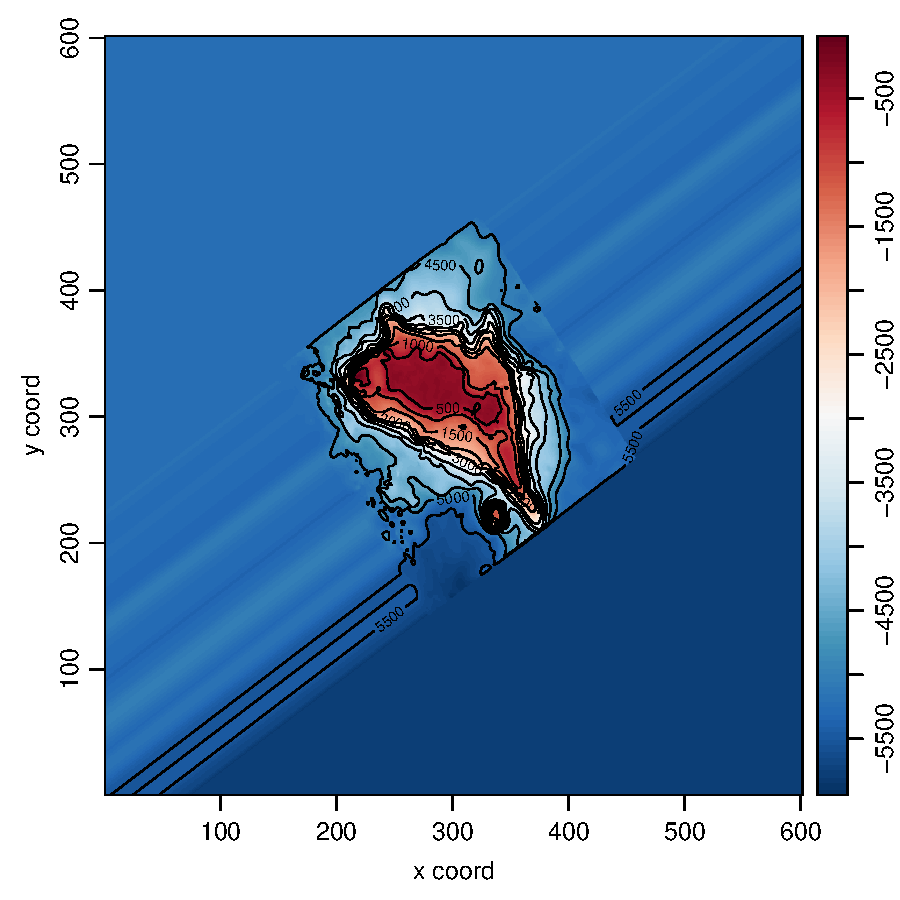
\includegraphics[scale=0.35]{../figures/kuril_bathy.pdf}
\caption{Three topography used in numerical investigations. a) Elliptical seamount with sharp skirt arises from 5500 m to 800 m. b) Real Koko guoyt topography cut from TOPO30 and turned $10^{\circ}$ to represent Japan case. c) Cut Koko guyot topography rotated by $35^{\circ}$ to represent Kuril case.}
\end{figure}
After reaching the stable regime the results were recorded and flux maps made. Also wave spectra decomposition was used to demodulate otherwise interfered signal.\\
The spatial resolution was the same and equal to $\delta x = \delta y = 1~km$. The time step for elliptical seamount experiment is $\delta t = 2~sec$ and for real topography cases $\delta t = 0.25~sec$.

\section{Simplified experiments}
\subsection{Circular seamount}
\begin{figure}
\centering
\includegraphics[scale=0.5]{../figures/test_seamount_bathy.png}
\caption{Circular seamount rising from 5300 m depth ocean up to 800 m.}
\end{figure}

\begin{figure}
\centering
\includegraphics[scale=0.5]{../figures/fluxes_circ_sm.png}
\caption{Energy fluxes for three experiments with different frequencies.}
\end{figure}

\begin{figure}
\centering
\includegraphics[scale=0.5]{../figures/spectra_windrose_circ_sm.png}
\caption{Directional distribution of wave energy for three experiments.}
\end{figure}

\bibliographystyle{apacite}
\bibliography{/home/dmitry/Bibtex_lib/}

\end{document}